\section{ТЕОРЕТИЧЕСКИЕ СВЕДЕНИЯ}
\label{sec:theory}

Существует большое количество различающихся по функциональному назначению сетевых утилит.
Необходимый набор сетевых утилит содержат современные операционные системы.
Так, например, «Служебные программы TCP/IP» Windows 2000
(см. «Справка» Windows 2000) состоят из трех групп-программ:
\begin{itemize}
\item служебные программы для обеспечения связи с удаленными узлами (Telnet, FTP, TFTP  и другие);
\item диагностические служебные программы для поиска и устранения сетевых неполадок;
\item серверное программное обеспечение TCP/IP (IIS, сервер печати TCP/IP, служба PWS).
\end{itemize}

Диагностические служебные программы Windows 2000 представляют собой утилиты командной строки.
Перечислим эти утилиты:
\begin{itemize}

\item ARP --- ARP отображает и изменяет локальные ARP-таблицы (таблицы соответствия MAC-адресов IP-адресам).

\item IPCONFIG --- отображает и изменяет сведения относящиеся конфигурации IP-адресов.
\item NETSTAT --- отображает сведения о текущих сетевых подключениях TCP/IP.
\item PING --- выполняет тестирование возможности соединения с указанным
    узлом и вычисляет период кругового обращения между источником и получателем.
\item PATHPING --- выполняет трассировку маршрута передаваемого пакета и выводит сведения о потерях пакетов.
\item ROUTE --- служит для отображения или изменения локальной таблицы маршрутизации.
\item TRACERT --- выполняет трассировку маршрута, по которому пакет доставляется получателю.
\item HOSTNAME --- выводит имя узла локального компьютера (используется без параметров).
\item NBTSTAT --- выводит таблицу имен NetBIOS, зарегистрированных локальными приложениями,
    и локальный кэш NetBIOS-имен, разрешенных в IP-адреса.
\item NSLOOKUP --- выводит записи, псевдонимы узлов домена,
    службы узлов домена и информацию об операционной системе, запрашивая DNS-серверы.
\item LPQ --- отображает сведения о состоянии удаленной очереди печати.

\end{itemize}

\pagebreak

\section{ХОД РАБОТЫ}

На рисунках~\ref{pic:arp}~--~\ref{pic:lpq} представлен вызов процедуры help для
приведенных в разделе~\ref{sec:theory} утилит.

\begin{figure}[h!]
  \centering
  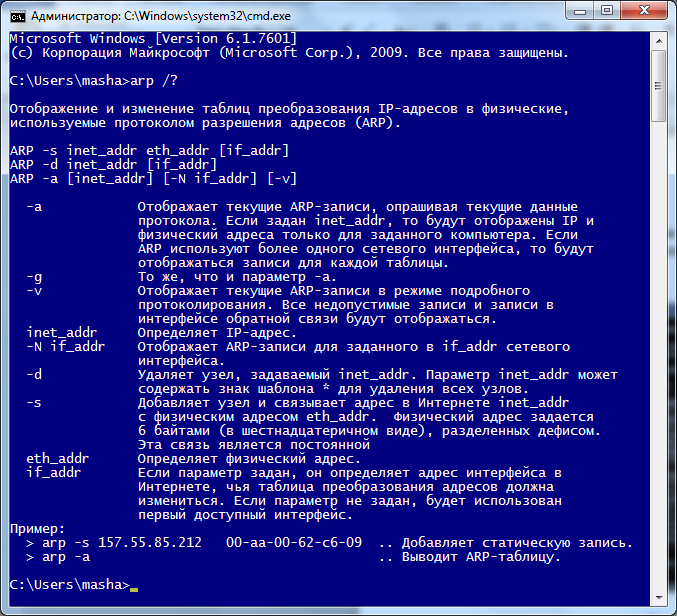
\includegraphics[width=0.6\linewidth]{pic/arp}
  \caption{Утилита \texttt{ARP}}
  \label{pic:arp}
\end{figure}

\begin{figure}[h!]
  \centering
  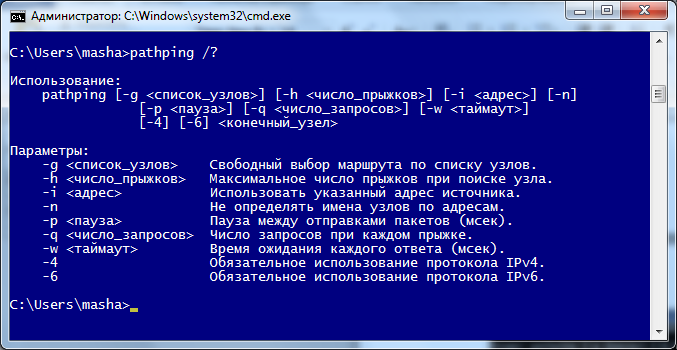
\includegraphics[width=0.9\linewidth]{pic/pathping}
  \caption{Утилита \texttt{PATHPING}}
  \label{pic:pathping}
\end{figure}

\newpage

\begin{figure}[h!]
  \centering
  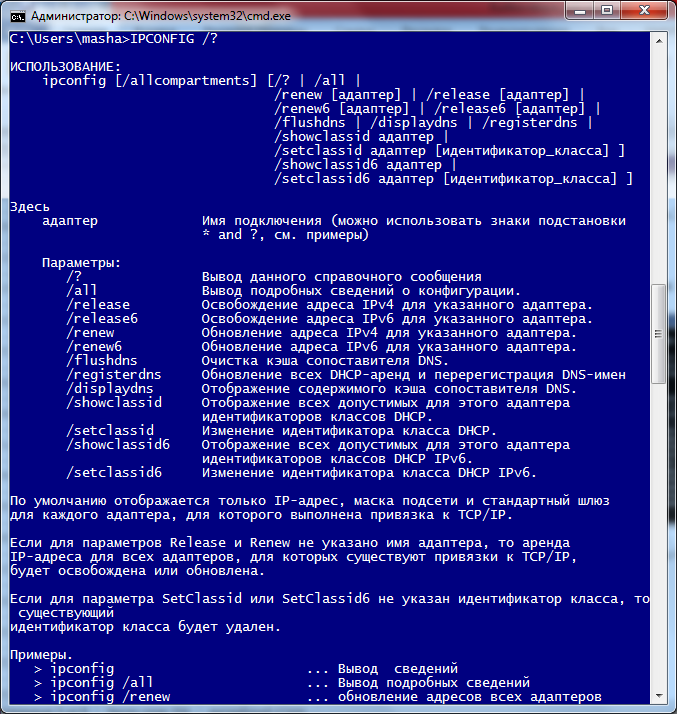
\includegraphics[width=0.6\linewidth]{pic/ipconfig}
  \caption{Утилита \texttt{IPCONFIG}}
  \label{pic:ipconfig}
\end{figure}

\begin{figure}[h!]
  \centering
  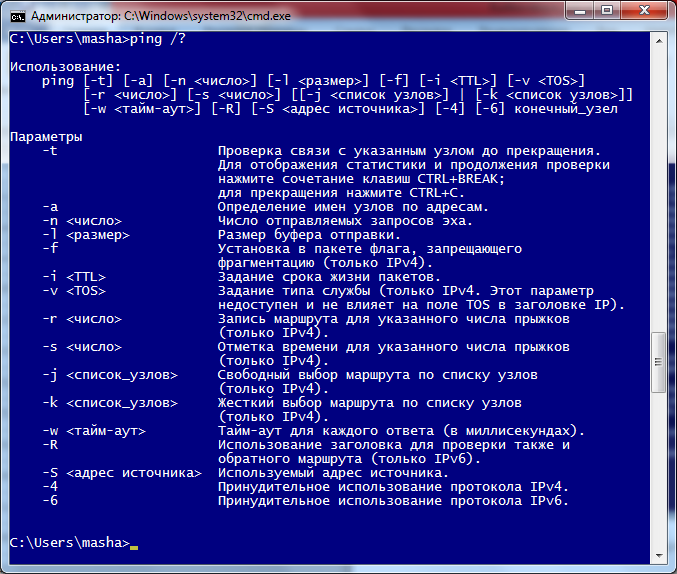
\includegraphics[width=0.7\linewidth]{pic/ping}
  \caption{Утилита \texttt{PING}}
  \label{pic:ping}
\end{figure}

\newpage

\begin{figure}[h!]
  \centering
  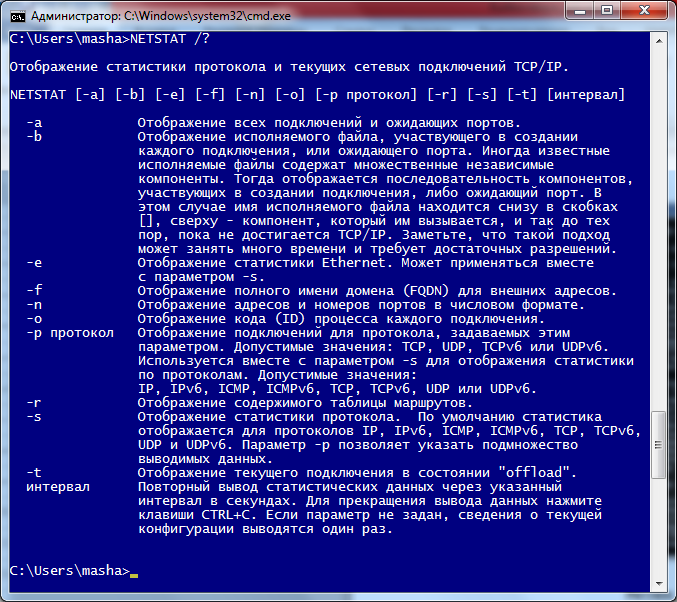
\includegraphics[width=0.9\linewidth]{pic/netstat}
  \caption{Утилита \texttt{NETSTAT}}
  \label{pic:netstat}
\end{figure}

\begin{figure}[h!]
  \centering
  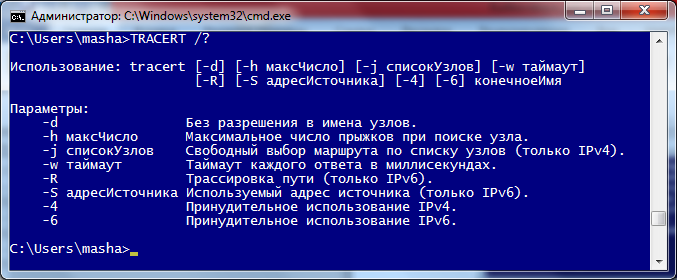
\includegraphics[width=0.9\linewidth]{pic/tracert}
  \caption{Утилита \texttt{TRACERT}}
  \label{pic:tracert}
\end{figure}

\newpage

\begin{figure}[h!]
  \centering
  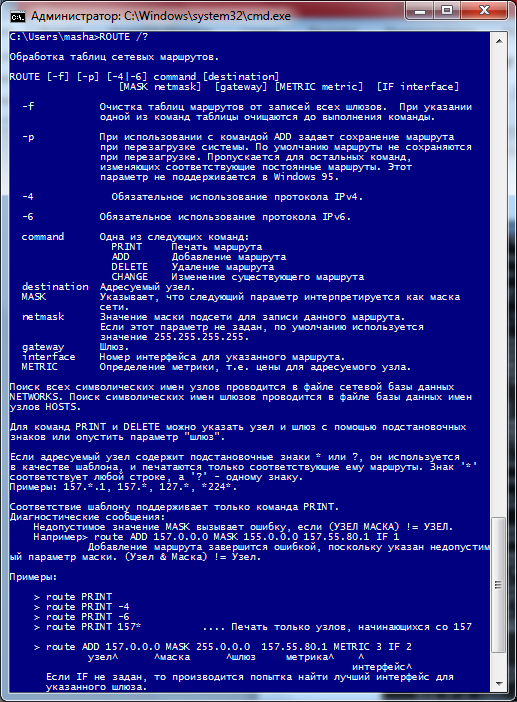
\includegraphics[width=1\linewidth]{pic/route}
  \caption{Утилита \texttt{ROUTE}}
  \label{pic:route}
\end{figure}

\newpage

\begin{figure}[h!]
  \centering
  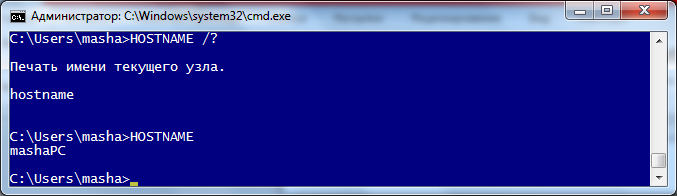
\includegraphics[width=0.8\linewidth]{pic/hostname}
  \caption{Утилита \texttt{HOSTNAME}}
  \label{pic:hostname}
\end{figure}

\begin{figure}[h!]
  \centering
  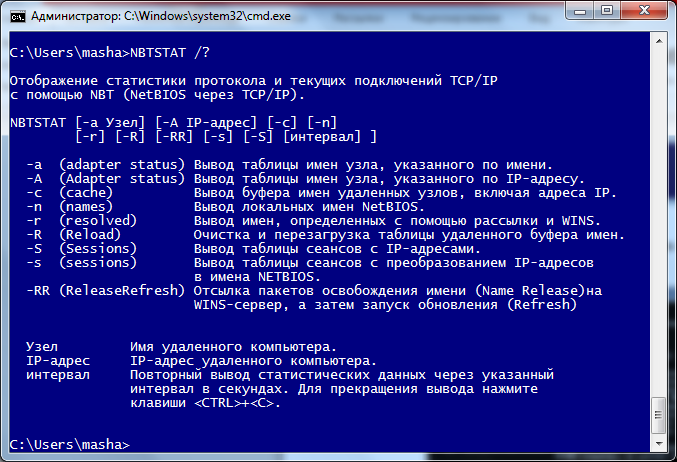
\includegraphics[width=0.8\linewidth]{pic/nbtstat}
  \caption{Утилита \texttt{NBTSTAT}}
  \label{pic:nbtstat}
\end{figure}

\begin{figure}[h!]
  \centering
  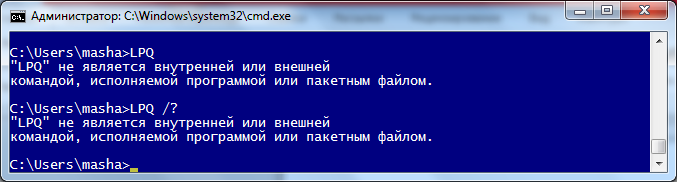
\includegraphics[width=0.8\linewidth]{pic/lpq}
  \caption{Утилита \texttt{LPQ}}
  \label{pic:lpq}
\end{figure}
